% Created 2023-04-21 Fri 20:48
% Intended LaTeX compiler: lualatex
\documentclass[11pt]{article}
\usepackage[margin=0.5in]{geometry}
\usepackage{syntax}
\usepackage{pdfpages}
\usepackage[most]{tcolorbox}
\usepackage{etoolbox}
\usepackage{environ}
\AtBeginEnvironment{quote}{\itshape}
\usepackage[ruled]{algorithm2e}
\let\oldtabular\tabular
\let\oldendtabular\endtabular
\NewEnviron{tabular2}[1]{\tcbox[left=0mm, right=0mm, top=0mm, bottom=0mm]{\oldtabular{#1}\BODY\oldendtabular}}
\usepackage{fontspec}
\setmonofont{JetBrainsMono Nerd Font Mono}[Renderer=Harfbuzz]
\BeforeBeginEnvironment{minted}{\begin{tcolorbox}[enhanced, breakable, skin first=enhanced, skin middle=enhanced, skin last=enhanced]}%
\AfterEndEnvironment{minted}{\end{tcolorbox}}
\BeforeBeginEnvironment{verbatim}{\begin{tcolorbox}[enhanced, breakable, skin first=enhanced, skin middle=enhanced, skin last=enhanced]}%
\AfterEndEnvironment{verbatim}{\end{tcolorbox}}
\usepackage{graphicx}
\usepackage{longtable}
\usepackage{wrapfig}
\usepackage{rotating}
\usepackage[normalem]{ulem}
\usepackage{amsmath}
\usepackage{amssymb}
\usepackage{capt-of}
\usepackage{hyperref}
\usepackage{minted}
\usepackage{physics}
\usepackage{pdfpages}
\usepackage{hyperref}
\hypersetup{colorlinks, linkcolor=blue}
\author{David Lewis}
\date{\today}
\title{}
\hypersetup{
 pdfauthor={David Lewis},
 pdftitle={},
 pdfkeywords={},
 pdfsubject={},
 pdfcreator={Emacs 30.0.50 (Org mode 9.6.1)}, 
 pdflang={English}}
\begin{document}

\setcounter{tocdepth}{2}
\tableofcontents


\section{Chapter 3}
\label{sec:org00bd418}

\subsection{UDP}
\label{sec:org02cb0a7}
\begin{itemize}
\item Checksum calculation
\end{itemize}

Binary addition of the source port + dest. port + length
\begin{center}
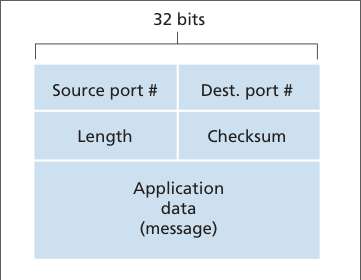
\includegraphics[width=0.7\textwidth]{checksum.png}
\end{center}

Carrying the one will wrap around to the beginning.

A handy python script I came up with:
\begin{minted}[fontsize=\scriptsize,breaklines=true,breakanywhere=true]{python}
# calculate checksum
def checksum(numbers):
    if len(numbers) > 3:
        print("this doesn't seem like udp")
    length = len(numbers[0])
    wrap = int("1" * length, 2)
    result = 0
    for i in numbers:
        i = int(i, 2)
        result += i
        if result > wrap:
            result -= wrap
    result = bin(result ^ wrap)[2:]
    result = (length-len(result)) * "0" + result
    return result
if __name__ == "__main__":
    print(checksum(["0110011001100000", "0101010101010101", "1000111100001100"]))
\end{minted}

\includepdf[pages=205-211, pagecommand={}]{computer-networking-a-top-down-approach-8th-edition.pdf}
\subsection{TCP}
\label{sec:org77660a2}
\subsubsection{fast retransmit}
\label{sec:org2a4cc54}
\begin{itemize}
\item If sender receives 3 duplicate acks, segment has been lost, segment is resent
before timer expires
\end{itemize}

\subsubsection{flow control}
\label{sec:orga152324}
\begin{itemize}
\item receive window is used to give the sender an idea of ho much free buffer
space is available.
\item UDP does not have flow control
\end{itemize}
\subsubsection{three way handshake}
\label{sec:orgb6c1969}
\begin{itemize}
\item client sends an initial segment (no payload), server sends an initial segment
as a reply (no payload), client sends another segment back (maybe payload)
\end{itemize}

\includepdf[pages=238-266, pagecommand={}]{computer-networking-a-top-down-approach-8th-edition.pdf}
\subsection{TCP congestion control}
\label{sec:org768684d}
\begin{itemize}
\item Slow start
:Initial sending rate is MSS/RTT (Max segment size/Round trip time), increases
congestion window by 1 MSS every acknowledged segment. Sending rate doubles
every RTT.
\item congestion avoidance: adds 1MSS each RTT
\item Fast recovery: Congestion window is increased by 1 MSS for every duplicate ACK
\item TCP Tahoe: Cut congestion window to 1 MSS and entered slow start
after either timout indicated or triple-duplicate ack loss event.
\item TCP Reno: incorporated fast recovery
\item AIMD (Additive increase Multiplicative-decrease): TCP congestion control, saw
tooth shape
\item TCP throughput: average throughput of a connection = \(\frac{0.75 \cdot W}{RTT}\)
\end{itemize}
\includepdf[pages=274-290, pagecommand={}]{computer-networking-a-top-down-approach-8th-edition.pdf}
\section{Chapter 4}
\label{sec:org31ed8b8}
\subsection{IP}
\label{sec:orgd17a22a}
\begin{itemize}
\item IPv4:
\begin{center}
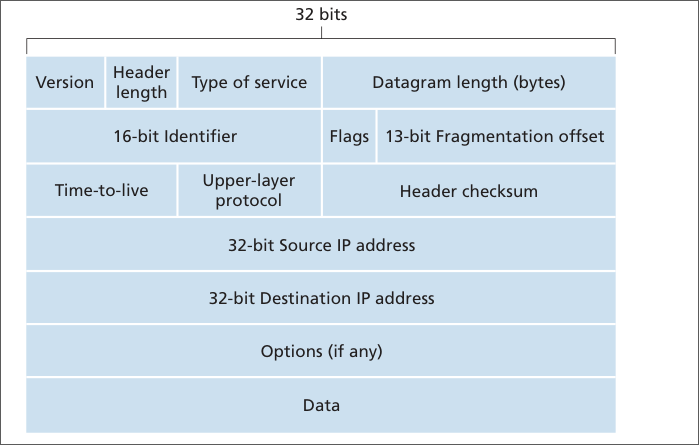
\includegraphics[width=0.7\textwidth]{datagram.png}
\end{center}
\item addressing: 32 bits long
\item subnetting: a subnet mask splits the IP address into two halves, the left of
which is the subnet mask address.
\item DHCP: dynamic host configuration protocol
\item NAT: network address translation
\item IPv6: \begin{center}
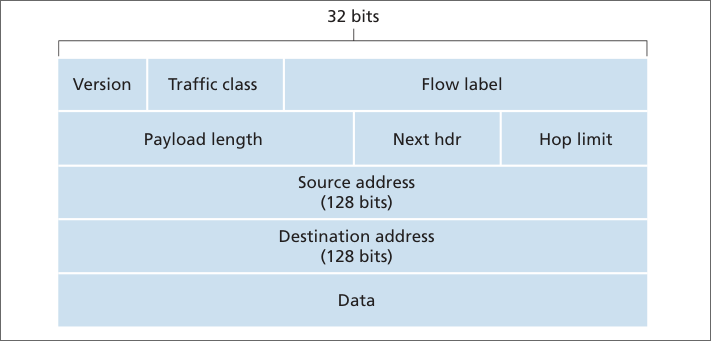
\includegraphics[width=0.7\textwidth]{datagram2.png}
\end{center}
\end{itemize}
\includepdf[pages=341-364, pagecommand={}]{computer-networking-a-top-down-approach-8th-edition.pdf}
\section{Chapter 5}
\label{sec:orgf8e2df1}
\subsection{Routing Algorithms}
\label{sec:org26ec236}
\begin{itemize}
\item link state (LS) routing - Dijkstra's algorithm
\item Distance-vector (DV) routing algorithm
\end{itemize}
\includepdf[pages=391-406, pagecommand={}]{computer-networking-a-top-down-approach-8th-edition.pdf}
\subsection{Intra-AS routing in the internet: OSPF}
\label{sec:org126fb77}
\includepdf[pages=406-410, pagecommand={}]{computer-networking-a-top-down-approach-8th-edition.pdf}
\subsection{ROuting among the ISPs: BGP}
\label{sec:org1505628}
\includepdf[pages=410-422, pagecommand={}]{computer-networking-a-top-down-approach-8th-edition.pdf}
\subsection{ICMP}
\label{sec:org0b1831d}
\includepdf[pages=434-436, pagecommand={}]{computer-networking-a-top-down-approach-8th-edition.pdf}
\section{Chapter 6}
\label{sec:org422acf2}
\subsection{Error-Detection and Correction techniques}
\label{sec:org18712f1}
\begin{itemize}
\item parity bits
\item CRC
\end{itemize}
\includepdf[pages=465-472, pagecommand={}]{computer-networking-a-top-down-approach-8th-edition.pdf}
\subsection{Switched Local Area Networks}
\label{sec:org520bc04}
\begin{itemize}
\item MAC addressing
\item ARP
\item self-learning mechanism of switches
\item switches vs routers vs hubs
\end{itemize}
\includepdf[pages=488-512, pagecommand={}]{computer-networking-a-top-down-approach-8th-edition.pdf}
\end{document}